\documentclass[11pt,a4paper,spanish]{book}
%\usepackage{estilo_unir}
\usepackage{biblatex}
\usepackage[utf8]{inputenc}
\usepackage{graphicx}
\graphicspath{ {./.images/} }
\usepackage{hyperref}
\usepackage{float}


\begin{document}

	
	\chapter{Objetivos y metodología de trabajo}
		
	\section{Objetivo General}
	
	\begin{enumerate}
		\item Conseguir un modelo que realice una clasificación emocional en el idioma de referencia escogido con un porcentaje de acierto por encima de un 80\%.
		\item Hacer un estudio comparativo del reconocimiento de emociones por voz, a través de lenguajes no aprendidos (lenguajes que no hayan formado parte del entrenamiento).
	\end{enumerate} 

	\section{Objetivos específicos}
	Para conseguir el alcance establecido, es necesario que los siguientes puntos sean satisfechos:
	\begin{itemize}
		\item Hacer un estudio del estado del arte sobre diferentes métodos, técnicas, y conjunto de datos utilizados en el reconocimiento de emociones a través de la voz. Aquí también se explorará si se dispone de la documentación necesaria, cómo cada uno de esos métodos pudiera estar relacionado con la lengua que usa para aplicarlo y su fonética.
		
		\item  Conseguir al menos 3 datasets pertenecientes a 3 idiomas diferentes donde uno de ellos será usado como referencia, y además, deberán cumplir las siguientes condiciones: Uno de los conjuntos de datos restantes deberá tener raíces fonéticas distintas al corpus de referencia, y el otro tener raíces fonéticas similares.
		
		\item Diseñar una solución en la que el conjunto de datos de referencia tenga un porcentaje de acierto del 80\% en la clasificación de emociones.
		
		\item Aplicar el modelo diseñado en el paso anterior a los otros conjuntos de datos.
		
		\item Evaluar la tasa de acierto obtenida en cada uno de eso conjuntos y comparar los resultados obtenidos.
		
	\end{itemize}
	\section{Metodología de trabajo}
	Para este proyecto se plantea una metodología de desarrollo iterativa, en las que tras una fase inicial, el proyecto entra en un bucle donde el producto pasa por una serie de etapas que se repiten durante la vida del proyecto. En cada iteración se diseñan unas modificaciones y capacidades funcionales que son añadidas al producto.
	
	\begin{enumerate}
		\item Fase inicial: Identifica el alcance del proyecto y los requisitos de una manera general pero lo suficientemente en detalle para que el tiempo y esfuerzo pueda ser estimado. Este paso inicial tiene como objetivo crear una versión del producto en la que se pueda trabajar como base (o mostrar a un cliente si lo hubiera)
		
		\item Elaboración: Se llevan a cabo los experimentos y la implementación de los componentes mediante unos pasos iterativos, a saber:
		
			\begin{enumerate}
				\item Planificación: Diseño del experimento o estudio que se quiere llevar a cabo teniendo en cuenta el tiempo disponible para ello, los posibles riesgos y el alcance deseado. Para ello se elabora una serie de tareas a implementar
				
				\item Implementación: Una vez identificadas las tareas en el paso anterior, se lleva a cabo la implementación del experimento.
				
				\item Evaluación: Se evalúan los resultados obtenidos de la implementación antes de decidir la iteración por finalizada. En caso de que los resultados no sean los esperados hay dos posibilidades: Si los errores obtenidos no distan demasiado de las especificaciones parciales, se pueden realizar reajustes en el modelo. Si por el contrario, dichos resultados están demasiado lejos del objetivo, se creará una segunda versión con una estrategia diferente, añadiendo más iteaciones al proceso de elaboración.
			\end{enumerate} 
		
		\item Despliegue: Es la etapa final, cuando el proyecto se da por finalizado.
	\end{enumerate}


	\begin{figure}[H]
		\centering
		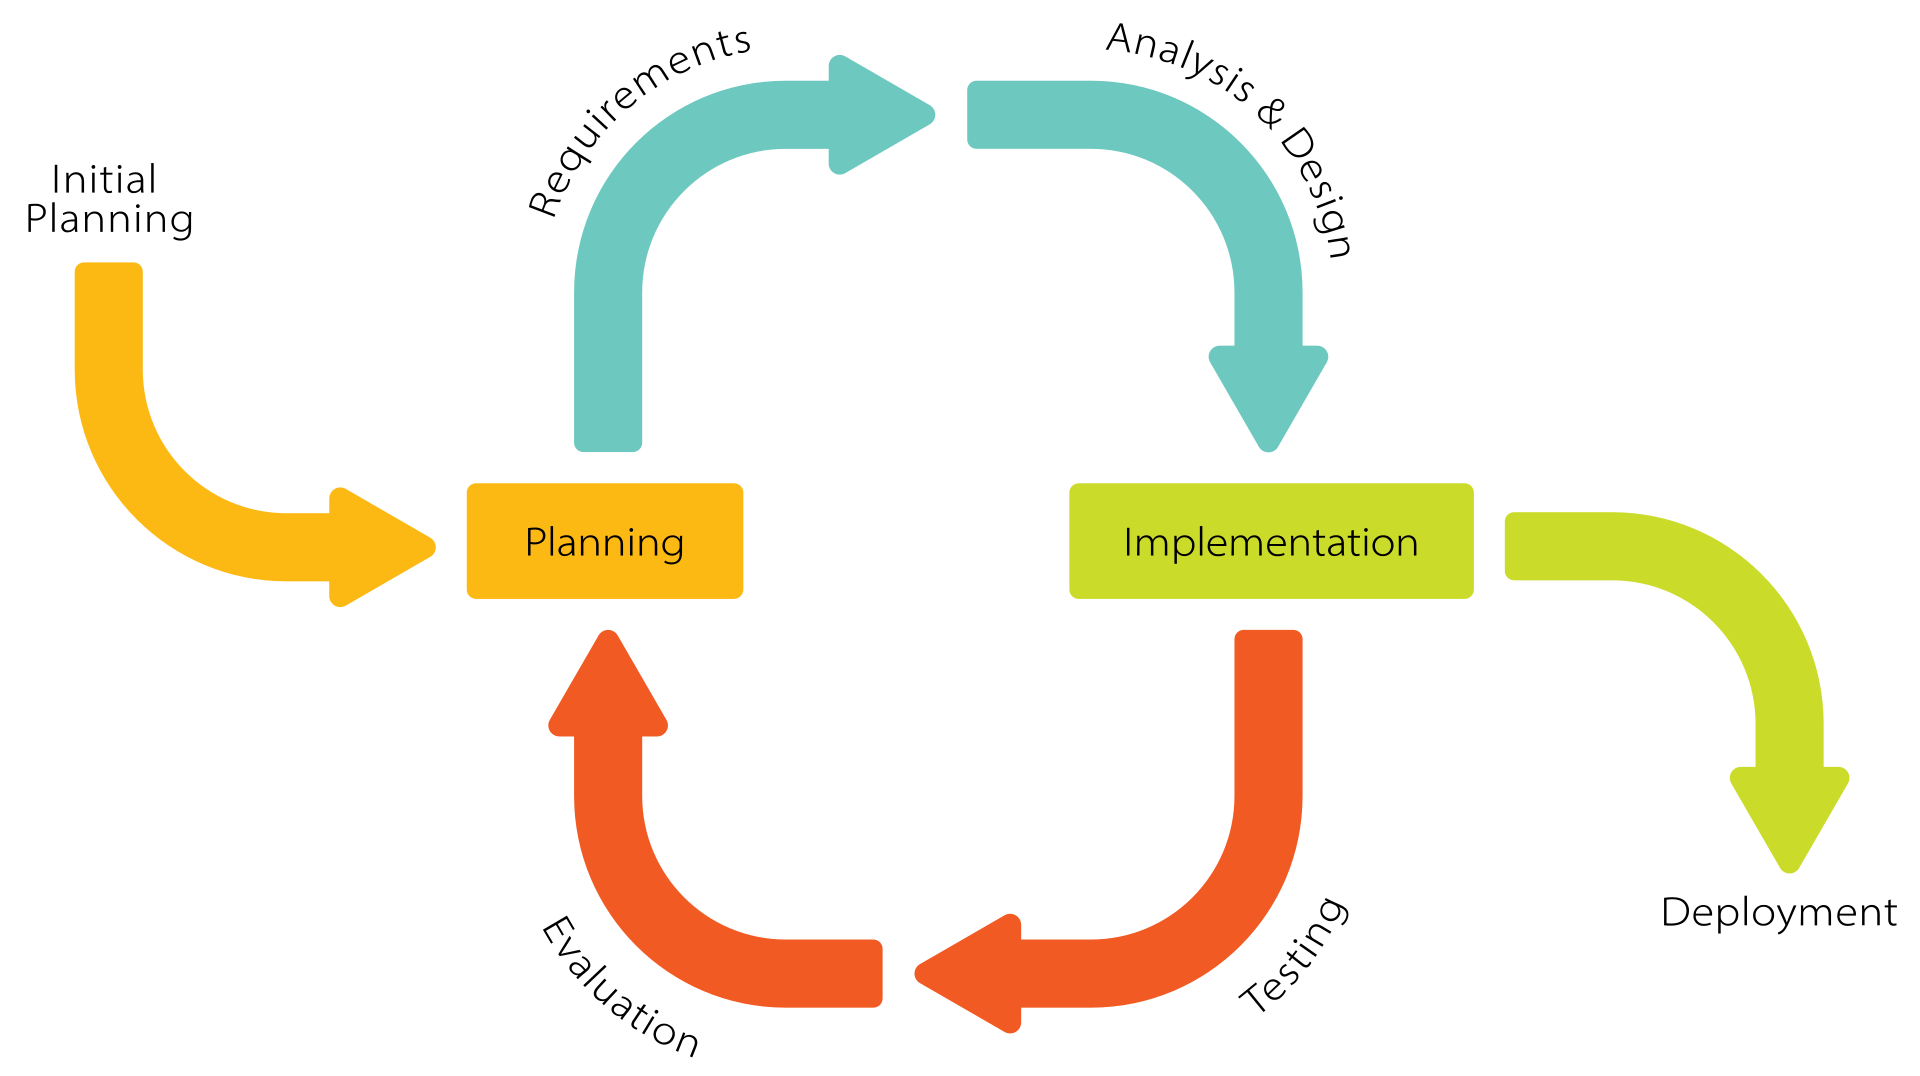
\includegraphics[scale=0.15]{Iterative_Process_Diagram.png}
		\caption{Proceso iterativo propuesto Fuente: \href{https://en.wikipedia.org/wiki/Iterative_and_incremental_development}{Wikipedia}}
		\label{fig:iterative_process}
	\end{figure}


		Al contrario que en desarrollos de software más tradicionales donde podrían verse flujos de trabajo basados en metodologías ágiles o en cascada, hemos creído que este modelo se adapta mejor a las necesidades de este proyecto, debido principalmente, al grado de incertidumbre que presenta un proyecto basado en Inteligencia Artificial en comparación con la ingeniería del software estándar. Por ejemplo, una metodología ágil asume que pequeños cambios funcionales hace posible el alcance de los objetivos a bajo coste y alta predictibilidad. Esto no se corresponde con este tipo de trabajo por las siguientes características:
		
		\begin{itemize}
			\item Es difícil conocer los costes y riesgos de la mayoría de los requisitos. Por ejemplo el estudio del conjunto de datos es algo que afecta directamente a la elaboración de los distintos modelos, y por lo tanto el crecimiento funcional es indeterminado.  
			
			\item Los cambios o modificaciones no pueden ser aplicados por diseño, requieren experimentos, además esas modificaciones son realmente complicadas de atomizar, por lo que el coste es impredecible. 
			
			\item Si bien es difícil tener una conclusión final por las estrictas fechas de entrega, un modelo iterativo permite obtener datos presentables a lo largo del proyecto.
		\end{itemize}
	
	
		
	
\end{document}